% !TeX program = xelatex
\documentclass[a4paper,10pt]{article}

% ============================================================================
% កញ្ចប់បណ្ណាល័យ (Packages) – តាមលំនាំ NGS Preah Krasang (ls_plan.tex)
% ============================================================================
\usepackage[a4paper, left=0.95cm, right=0.95cm, top=0.85cm, bottom=0.92cm, footskip=0.52cm]{geometry}
\usepackage{amsmath}
\usepackage{unicode-math}
\usepackage{fontspec}
\usepackage{array, longtable, multirow, colortbl}
\usepackage[table]{xcolor}
\usepackage{enumitem}
\usepackage{pifont}
\usepackage{fancyhdr}
\usepackage{tikz}
\usetikzlibrary{calc, arrows.meta, angles, quotes, decorations.markings, decorations.pathreplacing, patterns, babel}

% LaTeX 2025 + longtable v4.24 compatibility guard
\makeatletter
\let\@expl@@@mark@update@singlecol@structures@@\relax
\makeatother

% ============================================================================
% ការកំណត់ពុម្ពអក្សរ (Fonts Configuration - Cross-Platform Windows + Cloud fonts/)
% ============================================================================
\providecommand{\NGSFindFonts}{%
  \IfFileExists{C:/Windows/Fonts/cambria.ttc}{%
    \def\NGSSysPath{C:/Windows/Fonts/}%
    \def\NGSUserPath{C:/Users/KIT/AppData/Local/Microsoft/Windows/Fonts/}%
  }{%
    \IfFileExists{./fonts/KhmerOSsiemreap.ttf}{\def\NGSSysPath{./fonts/}\def\NGSUserPath{./fonts/}}{%
    \IfFileExists{../fonts/KhmerOSsiemreap.ttf}{\def\NGSSysPath{../fonts/}\def\NGSUserPath{../fonts/}}{%
    \IfFileExists{../../fonts/KhmerOSsiemreap.ttf}{\def\NGSSysPath{../../fonts/}\def\NGSUserPath{../../fonts/}}{%
    \IfFileExists{../../../fonts/KhmerOSsiemreap.ttf}{\def\NGSSysPath{../../../fonts/}\def\NGSUserPath{../../../fonts/}}{%
    \IfFileExists{../../../../fonts/KhmerOSsiemreap.ttf}{\def\NGSSysPath{../../../../fonts/}\def\NGSUserPath{../../../../fonts/}}{%
    \IfFileExists{../../../../../fonts/KhmerOSsiemreap.ttf}{\def\NGSSysPath{../../../../../fonts/}\def\NGSUserPath{../../../../../fonts/}}{%
    \IfFileExists{../../../../../../fonts/KhmerOSsiemreap.ttf}{\def\NGSSysPath{../../../../../../fonts/}\def\NGSUserPath{../../../../../../fonts/}}{%
      \def\NGSSysPath{../../../../../../../fonts/}\def\NGSUserPath{../../../../../../../fonts/}%
    }}}}}}}%
  }%
}
\NGSFindFonts

\setmathfont[
  Path={\NGSSysPath},
  FontIndex=1,
  Scale=1.02
]{cambria.ttc}

\defaultfontfeatures{Ligatures=TeX}

\setmainfont[
  Path={\NGSUserPath},
  Extension=.ttf,
  Script=Khmer,
  BoldFont={KhmerOSsiemreap},
  BoldFeatures={FakeBold=1.8},
  ItalicFont={KhmerOSsiemreap},
  ItalicFeatures={FakeSlant=0.25},
  BoldItalicFont={KhmerOSsiemreap},
  BoldItalicFeatures={FakeBold=1.8, FakeSlant=0.25}
]{KhmerOSsiemreap}

\newfontfamily\muol[
  Path={\NGSUserPath},
  Extension=.ttf,
  Script=Khmer
]{KhmerOSmuollight}

\newfontfamily\TimesEn[
  Path={\NGSSysPath},
  Extension=.ttf,
  Scale=1.00,
  BoldFont={timesbd},
  ItalicFont={timesi},
  BoldItalicFont={timesbi}
]{times}

\newfontfamily\NagaBold[
  Path={\NGSUserPath},
  Extension=.ttf
]{AKbalthom Naga Bold}

\newfontfamily\CalibriFont[
  Path={\NGSSysPath},
  Extension=.ttf
]{calibri}

\newfontfamily\Tacteing[
  Path={\NGSUserPath}
]{TACTENG.TTF}

\newfontfamily\CourierBullet[
  Path={\NGSSysPath},
  Extension=.ttf
]{cour}
\newcommand{\wcirc}{{\CourierBullet\fontsize{9.5pt}{11pt}\selectfont o}}

% ក្បួនកាត់ពាក្យខ្មែរ (Khmer word wrapping)
\XeTeXlinebreaklocale "km"
\XeTeXlinebreakskip = 0pt plus 1pt minus 0.1pt

% ============================================================================
% ការកំណត់ពណ៌ និងទម្រង់ទំព័រ (Colors & Page Style)
% ============================================================================
\definecolor{stepgray}{HTML}{D9D9D9}
\definecolor{headgray}{HTML}{F2F2F2}
\definecolor{boxgray}{HTML}{D9D9D9}
\definecolor{darkred}{HTML}{C00000}
\definecolor{red5e}{HTML}{FF0000}

\pagestyle{fancy}
\fancyhf{}
\renewcommand{\headrulewidth}{0pt}
\fancyfoot[R]{\CalibriFont\fontsize{11pt}{13pt}\selectfont\thepage}

\setlength{\parindent}{0pt}
\setlength{\parskip}{0pt}
\setlength{\tabcolsep}{3.8pt}

\newcolumntype{L}[1]{>{\raggedright\arraybackslash}p{#1}}

% ============================================================================
% ម៉ាក្រូជំនួយ (Helper Macros)
% ============================================================================
\newcommand{\en}[1]{{\TimesEn #1}}
\newcommand{\enbf}[1]{{\TimesEn\textbf{#1}}}
\newcommand{\unit}[1]{\,\text{\en{#1}}}
\newcommand{\fiveE}[1]{{\NagaBold\fontsize{9.5pt}{13pt}\selectfont\textcolor{red5e}{#1}}}
\newcommand{\timenote}[1]{\textcolor{darkred}{\textit{#1}}}
\newcommand{\redsub}[1]{\textcolor{darkred}{#1}}
\newcommand{\graybox}[1]{\colorbox{boxgray}{\strut\hspace{2pt}#1\hspace{2pt}}}
\newcommand{\ditem}{\tikz[baseline=-0.5ex]\fill (0,0.42ex) -- (0.42ex,0) -- (0,-0.42ex) -- (-0.42ex,0) -- cycle;\hspace{0.3em}}
\newcommand{\cnum}[1]{{\fontsize{10.5pt}{12pt}\selectfont\ding{\numexpr181+#1\relax}}\hspace{0.15em}}
\newcommand{\cfig}[1]{\par\vspace{4pt}{\centering #1\par}\vspace{4pt}}
\newcommand{\stepheader}[1]{\multicolumn{3}{|c|}{\cellcolor{stepgray}\muol #1} \\* \noalign{\hrule height 0.4pt}}
\newcommand{\fboxb}[1]{\begingroup\setlength{\fboxsep}{1.5pt}\fbox{#1}\endgroup}

% ក្បាច់ក្រោមបាវចនា (Tacteing Font - Keyboard '3')
\newcommand{\khmflourish}{{\Tacteing\fontsize{36pt}{14pt}\selectfont\raisebox{-5pt}{3}}}

% ============================================================================
% ម៉ាក្រូគូសរូប TikZ ស-ខ្មៅ ១០០% (Monochrome B&W TikZ Figures, Black Text, 6.2-6.8 cm)
% ============================================================================

% ១. ជំហានទី២ កំណែ & រំលឹក (p.16 ឃ. អន្ទាក់ស្វ័យគុណ ០ និង p.15 2^3*2^4=2^7)
\newcommand{\figStepTwoCheckEXP}{%
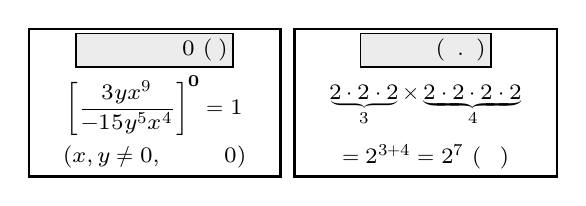
\begin{tikzpicture}[scale=0.90, every node/.style={font=\footnotesize, text=black}]
  % ឆ្វេង៖ អន្ទាក់ស្វ័យគុណ ០ នៃកន្សោមស្មុគស្មាញ
  \draw[black, line width=0.9pt] (0,0) rectangle (3.55,2.08);
  \node[fill=gray!15, draw=black, line width=0.6pt, inner sep=2pt] at (1.775,1.78) {អន្ទាក់ស្វ័យគុណ $0$ (ឃ)};
  \node at (1.775,1.00) {$\left[\dfrac{3yx^9}{-15y^5x^4}\right]^{\mathbf{0}} = 1$};
  \node at (1.775,0.28) {($x,y \neq 0$, ស្វ័យគុណ $0$)};
  % ស្ដាំ៖ រំលឹកគោលដូចគ្នា 2^3 * 2^4
  \draw[black, line width=0.9pt] (3.75,0) rectangle (7.45,2.08);
  \node[fill=gray!15, draw=black, line width=0.6pt, inner sep=2pt] at (5.60,1.78) {គោលដូចគ្នា (ទំ.១៥)};
  \node at (5.60,1.02) {$\underbrace{2\cdot 2\cdot 2}_{3}\times\underbrace{2\cdot 2\cdot 2\cdot 2}_{4}$};
  \node at (5.60,0.28) {$= 2^{3+4} = 2^7$ (បូក)};
\end{tikzpicture}}

% ២. E1 Engage: បន្ទះអង្គចងចាំ (2^3)^4 និងការ៉ូការេ (3b)^2
\newcommand{\figEngageMission}{%
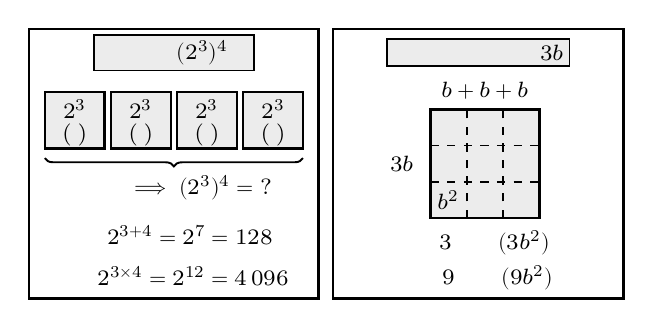
\begin{tikzpicture}[scale=1.0, every node/.style={font=\footnotesize, text=black}]
  % ស្ថានភាពទី១ (4.1): បន្ទះអង្គចងចាំ (2^3)^4 បៃ
  \draw[black, line width=0.95pt] (0,0) rectangle (3.68,3.42);
  \node[fill=gray!15, draw=black, line width=0.6pt, inner sep=2pt] at (1.84,3.12) {ស្ថានភាព ១៖ $(2^3)^4$ បៃ};
  \foreach \x/\lbl in {0.20/១, 1.04/២, 1.88/៣, 2.72/៤} {
    \draw[black, line width=0.85pt, fill=gray!15] (\x,1.90) rectangle (\x+0.76,2.62);
    \node at (\x+0.38,2.40) {$2^3$};
    \node at (\x+0.38,2.08) {(\lbl)};
  }
  \draw[black, line width=0.7pt, decorate, decoration={brace, mirror, amplitude=3pt}] (0.20,1.78) -- (3.48,1.78);
  \node at (1.84,1.40) {៤ បន្ទះ $\implies (2^3)^4 = ?$};
  \node at (1.84,0.80) {សុខ៖ $2^{3+4}=2^7=128$};
  \node at (1.84,0.28) {បូណា៖ $2^{3\times 4}=2^{12}=4\,096$};

  % ស្ថានភាពទី២ (4.2): ការ៉ូការេជ្រុង 3b
  \draw[black, line width=0.95pt] (3.86,0) rectangle (7.55,3.42);
  \node[fill=gray!15, draw=black, line width=0.6pt, inner sep=2pt] at (5.705,3.12) {ស្ថានភាព ២៖ ការ៉ូជ្រុង $3b$};
  \begin{scope}[shift={(5.10,1.02)}]
    \fill[gray!15] (0,0) rectangle (1.38,1.38);
    \draw[black, line width=0.95pt] (0,0) rectangle (1.38,1.38);
    \draw[black, line width=0.65pt, dashed] (0.46,0) -- (0.46,1.38) (0.92,0) -- (0.92,1.38);
    \draw[black, line width=0.65pt, dashed] (0,0.46) -- (1.38,0.46) (0,0.92) -- (1.38,0.92);
    \node at (-0.36,0.69) {$3b$};
    \node at (0.69,1.62) {$b+b+b$};
    \node[fill=gray!15, inner sep=0.5pt] at (0.23,0.23) {$b^2$};
  \end{scope}
  \node at (5.705,0.70) {សុខ៖ $3$ ការ៉ូ $(3b^2)$};
  \node at (5.705,0.26) {បូណា៖ $9$ ការ៉ូ $(9b^2)$};
\end{tikzpicture}}

% ៣. E2 Station 1 (POE 1 — 4.1): បន្ទះកញ្ចប់ ៤ នៃ 2^3 តម្រៀបបាន 12 កត្តា (2^{12} != 2^7)
\newcommand{\figPowerOfPowerStrip}{%
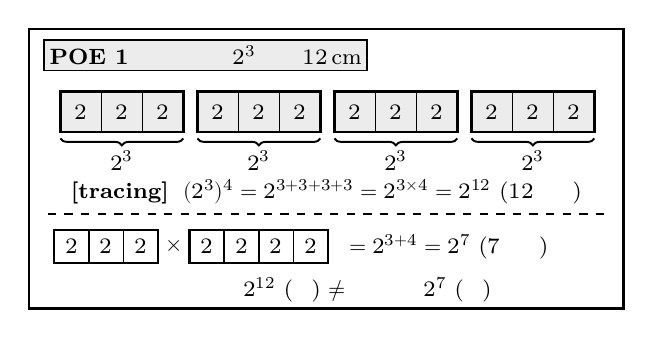
\begin{tikzpicture}[scale=1.0, every node/.style={font=\footnotesize, text=black}]
  \draw[black, line width=0.95pt] (0,0) rectangle (7.55,3.55);
  \node[anchor=north west, fill=gray!15, draw=black, line width=0.6pt, inner sep=2pt] at (0.18,3.42) {\textbf{POE 1៖} ៤ បន្ទះកញ្ចប់ $2^3$ លើថាស $12\unit{cm}$};

  % បន្ទះ ៤ ក្រុមនៃ 2*2*2
  \foreach \g in {0,1,2,3} {
    \pgfmathsetmacro{\gx}{0.40 + \g*1.74}
    \draw[black, line width=0.95pt, fill=gray!15] (\gx,2.24) rectangle (\gx+1.56,2.76);
    \draw[black, line width=0.6pt] (\gx+0.52,2.24) -- (\gx+0.52,2.76) (\gx+1.04,2.24) -- (\gx+1.04,2.76);
    \node at (\gx+0.26,2.50) {$2$};
    \node at (\gx+0.78,2.50) {$2$};
    \node at (\gx+1.30,2.50) {$2$};
    \draw[black, line width=0.7pt, decorate, decoration={brace, mirror, amplitude=2.5pt}] (\gx,2.16) -- (\gx+1.56,2.16);
    \node at (\gx+0.78,1.88) {$2^3$};
  }
  \node at (3.775,1.48) {\textbf{[tracing]}៖ $(2^3)^4 = 2^{3+3+3+3} = 2^{3\times 4} = 2^{12}$ ($12$ កត្តា)};

  % បន្ទះប្រៀបធៀបអន្ទាក់ 2^3 * 2^4 = 2^7
  \draw[black, line width=0.8pt, dashed] (0.24,1.20) -- (7.31,1.20);
  \draw[black, line width=0.9pt] (0.32,0.58) rectangle (1.64,1.00);
  \draw[black, line width=0.6pt] (0.76,0.58) -- (0.76,1.00) (1.20,0.58) -- (1.20,1.00);
  \node at (0.54,0.79) {$2$}; \node at (0.98,0.79) {$2$}; \node at (1.42,0.79) {$2$};
  \node at (1.84,0.79) {$\times$};
  \draw[black, line width=0.9pt] (2.04,0.58) rectangle (3.80,1.00);
  \draw[black, line width=0.6pt] (2.48,0.58) -- (2.48,1.00) (2.92,0.58) -- (2.92,1.00) (3.36,0.58) -- (3.36,1.00);
  \node at (2.26,0.79) {$2$}; \node at (2.70,0.79) {$2$}; \node at (3.14,0.79) {$2$}; \node at (3.58,0.79) {$2$};
  \node[anchor=west] at (3.94,0.79) {$= 2^{3+4} = 2^7$ ($7$ កត្តា)};
  \node at (3.775,0.24) {ឆ្លងវង់ក្រចក $2^{12}$ (គុណ) $\neq$ គោលដូចគ្នា $2^7$ (បូក)};
\end{tikzpicture}}

% ៤. E2 Station 2 (POE 2 — 4.2): ក្រឡា 3b x 3b = 9b^2 និងការ៉េបង្វិល 25° (2+3)^2 != 2^2+3^2
\newcommand{\figPowerOfProductArea}{%
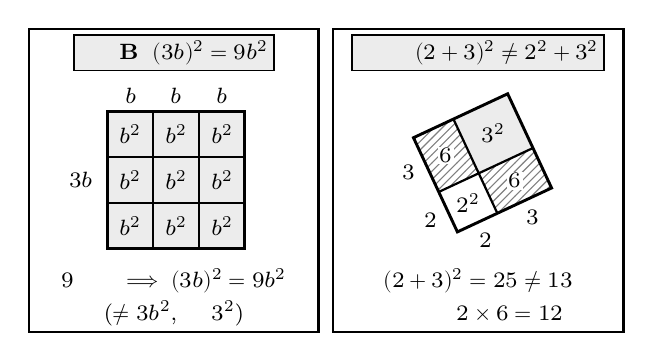
\begin{tikzpicture}[scale=1.0, every node/.style={font=\footnotesize, text=black}]
  % ផ្នែកឆ្វេង៖ ក្រឡា 3b x 3b = 9b^2
  \draw[black, line width=0.95pt] (0,0) rectangle (3.68,3.85);
  \node[fill=gray!15, draw=black, line width=0.6pt, inner sep=2pt] at (1.84,3.55) {\textbf{ផ្នែក \en{B}៖} $(3b)^2 = 9b^2$};
  \begin{scope}[shift={(1.00,1.06)}]
    \fill[gray!15] (0,0) rectangle (1.74,1.74);
    \draw[black, line width=1.05pt] (0,0) rectangle (1.74,1.74);
    \draw[black, line width=0.75pt] (0.58,0) -- (0.58,1.74) (1.16,0) -- (1.16,1.74);
    \draw[black, line width=0.75pt] (0,0.58) -- (1.74,0.58) (0,1.16) -- (1.74,1.16);
    \foreach \r in {0,1,2} {
      \foreach \c in {0,1,2} {
        \node at (\c*0.58+0.29, \r*0.58+0.29) {$b^2$};
      }
    }
    \node at (0.29,1.94) {$b$}; \node at (0.87,1.94) {$b$}; \node at (1.45,1.94) {$b$};
    \node at (-0.34,0.87) {$3b$};
  \end{scope}
  \node at (1.84,0.65) {$9$ ការ៉ូ $\implies (3b)^2=9b^2$};
  \node at (1.84,0.24) {($\neq 3b^2$, គុណ $3^2$)};

  % ផ្នែកស្ដាំ៖ អន្ទាក់លីនេអ៊ែរ ការ៉េបង្វិល 25° (2+3)^2 = 25 != 2^2 + 3^2 = 13
  \draw[black, line width=0.95pt] (3.86,0) rectangle (7.55,3.85);
  \node[fill=gray!15, draw=black, line width=0.6pt, inner sep=2pt] at (5.705,3.55) {\textbf{អន្ទាក់៖} $(2+3)^2 \neq 2^2+3^2$};
  \begin{scope}[shift={(5.76,2.15)}, rotate=25]
    \fill[white] (-0.66,-0.66) rectangle (-0.10,-0.10);
    \fill[gray!15] (-0.10,-0.10) rectangle (0.66,0.66);
    \fill[pattern=north east lines, pattern color=black!50] (-0.66,-0.10) rectangle (-0.10,0.66);
    \fill[pattern=north east lines, pattern color=black!50] (-0.10,-0.66) rectangle (0.66,-0.10);
    \draw[black, line width=1.05pt] (-0.66,-0.66) rectangle (0.66,0.66);
    \draw[black, line width=0.8pt] (-0.10,-0.66) -- (-0.10,0.66) (-0.66,-0.10) -- (0.66,-0.10);
    \node[fill=white, inner sep=0.5pt] at (-0.38,-0.38) {$2^2$};
    \node[fill=gray!15, inner sep=0.5pt] at (0.28,0.28) {$3^2$};
    \node[fill=white, inner sep=0.5pt] at (-0.38,0.28) {$6$};
    \node[fill=white, inner sep=0.5pt] at (0.28,-0.38) {$6$};
    \node at (-0.38,-0.90) {$2$};
    \node at (0.28,-0.90) {$3$};
    \node at (-0.90,-0.38) {$2$};
    \node at (-0.90,0.28) {$3$};
  \end{scope}
  \node at (5.705,0.65) {$(2+3)^2 = 25 \neq 13$};
  \node at (5.705,0.24) {បាត់ឆ្នូត $2\times 6=12$};
\end{tikzpicture}}

% ៥. E4 Elaborate: ស៊ុមវង់ក្រចកវិសាលភាព B&W [3]*[x^1]*[y^2] និង -2(a^{-3}b^5)^2 vs (-2a^{-3}b^5)^2
\newcommand{\figDetectiveScope}{%
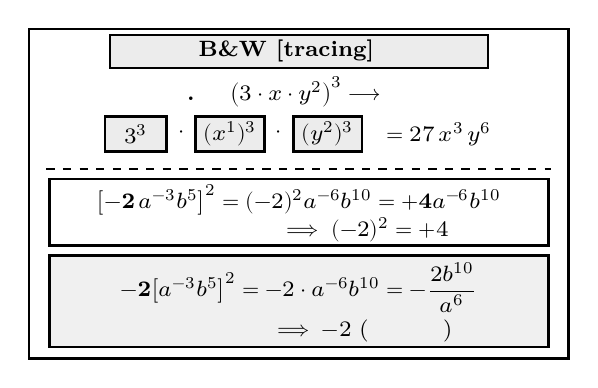
\begin{tikzpicture}[scale=0.92, every node/.style={font=\footnotesize, text=black}]
  \draw[black, line width=0.95pt] (0,0) rectangle (7.45,4.55);
  \node[fill=gray!15, draw=black, line width=0.6pt, inner sep=2pt] at (3.725,4.24) {\textbf{សញ្ញាសម្គាល់ \en{B\&W} [tracing] វិសាលភាពវង់ក្រចក}};

  % ជួរលើ៖ (3xy^2)^3
  \node at (3.725,3.68) {\textbf{គំរូ ៤.២ ក៖} $\big(3\cdot x\cdot y^2\big)^3 \longrightarrow$ បំបែកកត្តា};
  \draw[black, line width=0.85pt, fill=gray!15] (1.05,2.86) rectangle (1.90,3.34);
  \node at (1.475,3.10) {$3^3$};
  \node at (2.10,3.10) {$\cdot$};
  \draw[black, line width=0.85pt, fill=gray!15] (2.30,2.86) rectangle (3.25,3.34);
  \node at (2.775,3.10) {$(x^1)^3$};
  \node at (3.45,3.10) {$\cdot$};
  \draw[black, line width=0.85pt, fill=gray!15] (3.65,2.86) rectangle (4.60,3.34);
  \node at (4.125,3.10) {$(y^2)^3$};
  \node[anchor=west] at (4.80,3.10) {$= 27\,x^3\,y^6$};

  \draw[black, line width=0.75pt, dashed] (0.24,2.62) -- (7.21,2.62);

  % ជួរក្រោម៖ កាត ២ ជាន់ (ច្បាស់ ១០០% គ្មានជាន់គ្នា)
  \draw[black, line width=0.9pt] (0.28,1.56) rectangle (7.17,2.48);
  \node at (3.725,2.18) {$\big[\mathbf{-2}\,a^{-3}b^5\big]^2 = (-2)^2 a^{-6}b^{10} = \mathbf{+4}a^{-6}b^{10}$};
  \node at (3.725,1.78) {\textbf{សញ្ញាដកក្នុងវង់ក្រចក} $\implies (-2)^2 = +4$};

  \draw[black, line width=0.95pt, fill=gray!12] (0.28,0.16) rectangle (7.17,1.42);
  \node at (3.725,0.98) {$\mathbf{-2}\big[a^{-3}b^5\big]^2 = -2\cdot a^{-6}b^{10} = -\dfrac{2b^{10}}{a^6}$};
  \node at (3.725,0.38) {\textbf{សញ្ញាដកក្រៅវង់ក្រចក} $\implies -2$ (រក្សាសញ្ញាដក)};
\end{tikzpicture}}

% ៦. E5 Exit Foils A–D (Printable ទំព័រ ៥)
\newcommand{\figExitCardsEXP}{%
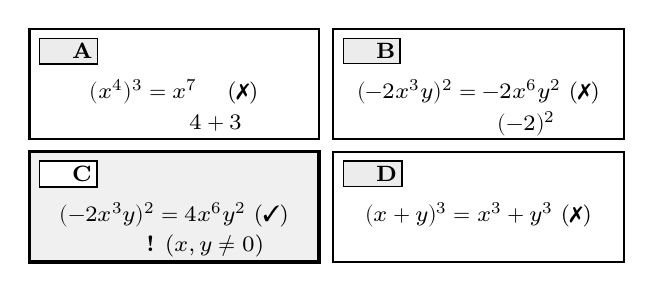
\begin{tikzpicture}[scale=1.0, every node/.style={font=\footnotesize, text=black}]
  % A (X)
  \draw[black, line width=0.9pt] (0,1.56) rectangle (3.68,2.96);
  \node[anchor=north west, fill=gray!15, draw=black, line width=0.6pt, inner sep=1.8pt] at (0.12,2.85) {\textbf{កាត \en{A}}};
  \node at (1.84,2.16) {$(x^4)^3 = x^7$ \quad (\ding{55})};
  \node at (1.84,1.76) {អន្ទាក់៖ បូក $4+3$};

  % B (X)
  \draw[black, line width=0.9pt] (3.86,1.56) rectangle (7.55,2.96);
  \node[anchor=north west, fill=gray!15, draw=black, line width=0.6pt, inner sep=1.8pt] at (3.98,2.85) {\textbf{កាត \en{B}}};
  \node at (5.705,2.16) {$(-2x^3y)^2 = -2x^6y^2$ (\ding{55})};
  \node at (5.705,1.76) {អន្ទាក់៖ ភ្លេច $(-2)^2$};

  % C (CHECK)
  \draw[black, line width=1.15pt, fill=gray!12] (0,0) rectangle (3.68,1.40);
  \node[anchor=north west, fill=white, draw=black, line width=0.6pt, inner sep=1.8pt] at (0.12,1.29) {\textbf{កាត \en{C}}};
  \node at (1.84,0.60) {$(-2x^3y)^2 = 4x^6y^2$ (\ding{51})};
  \node at (1.84,0.20) {\textbf{ត្រឹមត្រូវ!} ($x,y\neq 0$)};

  % D (X)
  \draw[black, line width=0.9pt] (3.86,0) rectangle (7.55,1.40);
  \node[anchor=north west, fill=gray!15, draw=black, line width=0.6pt, inner sep=1.8pt] at (3.98,1.29) {\textbf{កាត \en{D}}};
  \node at (5.705,0.60) {$(x+y)^3 = x^3+y^3$ (\ding{55})};
  \node at (5.705,0.20) {អន្ទាក់៖ បំបែកលើផលបូក};
\end{tikzpicture}}

% ============================================================================
% ចាប់ផ្ដើមឯកសារ (Document Body)
% ============================================================================
\begin{document}
\fontsize{10pt}{15.2pt}\selectfont

% -------------------- ក្បាលកិច្ចតែងការ (Header) --------------------
\begin{center}
  {\muol\fontsize{11pt}{16pt}\selectfont ព្រះរាជាណាចក្រកម្ពុជា}\\[2pt]
  {\muol\fontsize{10pt}{15pt}\selectfont ជាតិ សាសនា ព្រះមហាក្សត្រ}\\[1pt]
  \khmflourish
\end{center}

\vspace{-26pt}
{\muol\fontsize{9.5pt}{12.5pt}\selectfont
មន្ទីរអប់រំ យុវជន និងកីឡា ខេត្តកំពង់ធំ\\
ការិយាល័យអប់រំ យុវជន និងកីឡា ស្រុកកំពង់ស្វាយ\\
អនុវិទ្យាល័យព្រះក្រសាំង}

\vspace{1pt}
\begin{center}
  {\muol\fontsize{10pt}{14pt}\selectfont កិច្ចតែងការបង្រៀន}
\end{center}
\vspace{0pt}

% -------------------- ព័ត៌មានទូទៅ (Metadata) --------------------
{\renewcommand{\arraystretch}{0.98}
\hspace*{3.4cm}%
\begin{tabular}{@{}l l L{10.5cm}@{}}
  - \hspace{0.35cm} មុខវិជ្ជា & : & គណិតវិទ្យា ថ្នាក់ទី៨ (ពីជគណិត) \\
  - \hspace{0.35cm} ចំណងជើងមេរៀន & : & មេរៀនទី២៖ ស្វ័យគុណ \\
  - \hspace{0.35cm} ចំណងជើងរង & : & ២.៤.១. ស្វ័យគុណនៃស្វ័យគុណ និង ២.៤.២. ស្វ័យគុណនៃផលគុណ (ទំព័រ ១៧–១៨ ដើម) \\
  - \hspace{0.35cm} រយៈពេល & : & ១ ម៉ោងសិក្សា (៥០នាទី) \\
  - \hspace{0.35cm} បង្រៀនដោយ & : & ហុក ប៊ុនថែន \\
  - \hspace{0.35cm} កាលបរិច្ឆេទ & : & \makebox[28mm]{\dotfill}\ ២០២៦ \\
\end{tabular}

\vspace{2pt}

% -------------------- I. វត្ថុបំណង --------------------
\textbf{I.} {\muol វត្ថុបំណង}\\[1pt]
\hspace*{0.55cm}%
\begin{tabular}{@{}l l L{14.2cm}@{}}
  \wcirc \hspace{0.25cm} វិជ្ជាសម្បទា & : & សិស្សបង្គុំនិងប្រាប់រូបមន្តស្វ័យគុណនៃស្វ័យគុណ $(a^m)^n = (a^n)^m = a^{m\cdot n}$ (៤.១) និងស្វ័យគុណនៃផលគុណ $(a\cdot b)^n = a^n\cdot b^n$ និងទម្រង់បញ្ច្រាស $a^n\cdot b^n = (ab)^n$ (៤.២) ដោយបញ្ជាក់លក្ខខណ្ឌ $a\neq 0, b\neq 0$ ពេលនិទស្សន្ត $\le 0$ ។ \\
  \wcirc \hspace{0.25cm} បំណិនសម្បទា & : & សិស្សអនុវត្តពិសោធន៍ \en{Dual POE 1:1} (បន្ទះ $(2^3)^4$ និងក្រឡា $(3b)^2$ ធៀប $(2+3)^2$), ប្រើ \textbf{[tracing]}, វង់ក្រចកវិសាលភាព \en{[3]$\cdot$[x$^1$]$\cdot$[y$^2$]} និង \cnum{1}--\cnum{5} គណនាលំហាត់គំរូ ប្រតិបត្តិ ទំ.១៧–១៨ ដើម និងកិច្ចការផ្ទះ ទំ.២៥–២៦ បានត្រឹមត្រូវ ។ \\
  \wcirc \hspace{0.25cm} ចរិយាសម្បទា & : & សហការក្នុងក្រុម ៣ នាក់តាមវិធី \en{Relay} ៣ តួនាទីដោយគោរពវិន័យ \en{Pause-Ask / Pause-Review} និងប្រុងប្រយ័ត្នចំពោះអន្ទាក់សញ្ញាដកក្រៅវង់ក្រចកនិងការបំបែកលើផលបូក ។ \\
\end{tabular}

\vspace{2pt}

% -------------------- II. សម្ភារៈឧបទេស --------------------
\textbf{II.} {\muol សម្ភារៈឧបទេស}\\[1pt]
\hspace*{0.55cm}$\bullet$ \hspace{0.35cm} សៀវភៅគោលទី៨ (ទំ.១៦–១៨ ដើម, ២៥–២៦) បន្ទាត់ក្រិត ១:១ កន្ត្រៃ ខ្មៅដៃគូស \textbf{[tracing]} កញ្ចប់ ១:១ (ទំព័រ ១) កាត \en{E4} (ទំព័រ ២) សន្លឹក \en{Relay E5} (ទំព័រ ៣) ផ្ទាំង \cnum{1}--\cnum{5} (ទំព័រ ៤) កាត \en{A--D} (ទំព័រ ៥) និងប័ណ្ណកិច្ចការផ្ទះ (ទំព័រ ៦)

\vspace{2pt}

% -------------------- III. វិធីសាស្រ្តបង្រៀន --------------------
\textbf{III.} {\muol វិធីសាស្រ្តបង្រៀន}\\[1pt]
\hspace*{0.45cm}%
\begin{tabular}{@{}l l L{14.85cm}@{}}
  $\bullet$ \hspace{0.25cm} គោលវិធី & : & សិស្សមជ្ឈមណ្ឌល \\
  $\bullet$ \hspace{0.25cm} យុទ្ធវិធីបង្រៀន & : & ស្ថាបនានិយម គំរូ \en{5Es} (កាត់បន្ទះ \en{1:1}, \en{Dual POE}, \textbf{[tracing]}, វង់ក្រចក \en{B\&W}, \en{Relay} ៣ តួនាទី) \\
\end{tabular}
}

\vspace{2pt}

% -------------------- IV. ដំណើរការបង្រៀន --------------------
\textbf{IV.} {\muol ដំណើរការបង្រៀន}

\vspace{1pt}

% ============================================================================
% តារាងដំណើរការបង្រៀន (Granular 2-5 Line Sub-Rows, Dedicated TikZ Rows, 50 min)
% ============================================================================
\renewcommand{\arraystretch}{1.15}
\begin{longtable}{|L{5.50cm}|L{7.90cm}|L{4.80cm}|}
\hline
\rowcolor{headgray}
\multicolumn{1}{|c|}{\muol សកម្មភាពគ្រូ} &
\multicolumn{1}{c|}{\muol ខ្លឹមសារមេរៀន} &
\multicolumn{1}{c|}{\muol សកម្មភាពសិស្ស} \\
\hline
\endfirsthead

\hline
\endhead

\hline
\endfoot

\hline
\endlastfoot

% ==================== ជំហានទី១ (2min) ====================
\stepheader{ជំហានទី១ \enbf{(}រដ្ឋបាលថ្នាក់\enbf{)}}
$\bullet$ ពិនិត្យអវត្តមាន អនាម័យ និងសណ្ដាប់ធ្នាប់ថ្នាក់រៀន
&
$\bullet$ រដ្ឋបាលថ្នាក់ \par
$\bullet$ អនាម័យ និងវិន័យសុវត្ថិភាពកន្ត្រៃ
&
$\circ$ ប្រធានថ្នាក់រាយការណ៍អវត្តមាន \\[3pt]

$\bullet$ រៀបចំសិស្សជាក្រុម ៣ នាក់ («ក្រុមវិស្វករអង្គចងចាំ និងការ៉ូ ៣ តួនាទី») \par
$\bullet$ ចែកកញ្ចប់ ១:១ (\en{Printable} ទំព័រ ១) ផ្កាប់លើតុ
&
$\bullet$ ត្រៀមក្រុម ៣ នាក់ និងរៀបចំសម្ភារៈ \en{B\&W} (កន្ត្រៃ បន្ទាត់ ១:១ ខ្មៅដៃ)
&
$\circ$ អង្គុយតាមក្រុម ៣ នាក់ និងដាក់សន្លឹក ១:១ ផ្កាប់លើតុ \\
\hline

% ==================== ជំហានទី២ (9min: <=3 + 3 + E1 3) ====================
\stepheader{ជំហានទី២ \enbf{(}កិច្ចការផ្ទះ \enbf{+} ទំនាក់ទំនងមេរៀនថ្មី\enbf{)}}
% --- ២.១ កំណែកិច្ចការផ្ទះ (<=3min) ---
\ditem \textbf{កំណែកិច្ចការផ្ទះ ($\le 3\unit{min}$)} \timenote{(កុំសរសេរវែង)} \par
$\bullet$ ហៅសិស្សផ្ទៀង \textbf{ប្រតិបត្តិ ទំ.១៦ (ក, ខ)}
&
{\centering\redsub{កំណែកិច្ចការផ្ទះមេរៀនមុន (ប្រតិបត្តិ ទំ.១៦)}\par} \par
$\bullet$ \textbf{ក.} $\dfrac{x^9}{x^4} = x^{9-4} = x^5$ ($x \neq 0$) \par
$\bullet$ \textbf{ខ.} $\dfrac{(3/2)^2}{(3/2)^4} = \left(\dfrac{3}{2}\right)^{2-4} = \left(\dfrac{3}{2}\right)^{-2} = \dfrac{4}{9}$
&
$\circ$ ផ្ទៀងចម្លើយ \textbf{ក, ខ} លើក្ដារខៀន និងកែតម្រូវក្នុងសៀវភៅ \\[3pt]

$\bullet$ ហៅសិស្សផ្ទៀង \textbf{គ, ឃ} និងសួរអន្ទាក់ស្វ័យគុណ $0$ \par
\hspace*{0.3em}– \textbf{សំណួរ៖} «ក្នុងលំហាត់ \textbf{ឃ} តើចាំបាច់សម្រួលក្នុងវង់ក្រចកមុនលើកស្វ័យគុណ $0$ ទេ?»
&
$\bullet$ \textbf{គ.} $\dfrac{y^9}{y^9} = y^0 = 1$ ($y \neq 0$) \par
$\bullet$ \textbf{ឃ.} $\left(\dfrac{3yx^9}{-15y^5x^4}\right)^0 = 1$ ($x, y \neq 0$)
&
$\circ$ ឆ្លើយ៖ «កន្សោមខុសពី $0$ ទាំងមូលស្វ័យគុណ $0$ ស្មើ $1$ ភ្លាម!» \\[3pt]

&
\cfig{\figStepTwoCheckEXP}
& \\[3pt]

% --- ២.២ រំលឹកមេរៀនចាស់ (3min) ---
\ditem \textbf{រំលឹកមេរៀនចាស់ (3min)} \par
$\bullet$ សួរនិយមន័យស្វ័យគុណ អវិជ្ជមាន និងផលគុណគោលដូចគ្នា (ទំ.១៥) \par
\hspace*{0.3em}– \textbf{សំណួរ៖} «បើគោលដូចគ្នាគុណគ្នា ($2^3 \cdot 2^4$) តើធ្វើដូចម្ដេចនឹងនិទស្សន្ត?»
&
{\centering\redsub{រំលឹកមេរៀនទាក់ទងមេរៀនថ្មី}\par} \par
$\bullet$ $a^n = \underbrace{a\cdot a\cdots a}_{n\text{ កត្តា}}$ និង $a^{-n} = \dfrac{1}{a^n}$ ($a \neq 0$) \par
$\bullet$ $a^m \cdot a^n = a^{m+n}$ \quad (ឧ. $2^3 \cdot 2^4 = 2^7$, ទំ.១៥)
&
$\circ$ ឆ្លើយ៖ «រក្សាគោលដដែល រួចបូកនិទស្សន្ត ($2^{3+4} = 2^7$)» \\[3pt]

% --- ២.៣ E1 Engage (3min) ---
\fiveE{E1 - Engage (3min)} \timenote{(កុំទាន់ផ្ដល់ចម្លើយ)} \par
\ditem \textbf{បេសកកម្មទី១ (៤.១)៖} អង្គចងចាំកុំព្យូទ័រពង្រីក ៤ តំណាក់កាល $(2^3)^4$ បៃ \par
\hspace*{0.3em}– \textbf{សំណួរ៖} «តើសុខ ($2^7=128$) ឬបូណា ($2^{12}=4\,096$) ត្រូវ?»
&
{\centering\redsub{បេសកកម្ម E1៖ បន្ទះអង្គចងចាំ និងការ៉ូការេពង្រីកខ្នាត}\par} \par
$\bullet$ \textbf{ស្ថានភាពទី១ (៤.១)៖} កញ្ចប់ទិន្នន័យ $(2^3)^4$ បៃ \par
$\bullet$ សុខថា៖ $(2^3)^4 = 2^{3+4} = 2^7 = 128$ \par
$\bullet$ បូណាថា៖ $(2^3)^4 = 2^{3\times 4} = 2^{12} = 4\,096$
&
$\circ$ សង្កេតស្ថានភាពទី១ និងទស្សន៍ទាយខាងសុខ ឬបូណា \\[3pt]

&
\cfig{\figEngageMission}
& \\[3pt]

\ditem \textbf{បេសកកម្មទី២ (៤.២)៖} ការេធំជ្រុង $(3b)\unit{cm}$ ផ្សំពីការ៉ូតូចជ្រុង $b\unit{cm}$ \par
\hspace*{0.3em}– \textbf{សំណួរ៖} «តើត្រូវការការ៉ូតូច $3b^2$ ឬ $9b^2$?»
&
$\bullet$ \textbf{ស្ថានភាពទី២ (៤.២)៖} ការេធំជ្រុង $(3b)\unit{cm}$ ផ្សំពីការ៉ូជ្រុង $b\unit{cm}$ \par
$\bullet$ សុខថា៖ $(3b)^2 = 3b^2$ ($3$ ការ៉ូ) \quad \textbar{} \quad បូណាថា៖ $(3b)^2 = 9b^2$ ($9$ ការ៉ូ)
&
$\circ$ ស្រង់ការទស្សន៍ទាយក្រុមទុកលើក្ដារខៀន (មិនទាន់បញ្ជាក់) \\
\hline

% ==================== ជំហានទី៣ (17min: E2 11m + E3 6m) ====================
\stepheader{ជំហានទី៣ \enbf{(}ខ្លឹមសារមេរៀនថ្មី\enbf{)}}
% --- ៣.១ ចំណងជើង & E2 Explore Station 1 (5min) ---
\fiveE{E2 - Explore (11min)} \par
$\bullet$ សរសេរចំណងជើងមេរៀនលើក្ដារខៀន
&
មេរៀនទី២ \hspace{0.15cm} {\muol ស្វ័យគុណ} \textbf{(ត)} \par
\textbf{៤. លក្ខណៈនៃស្វ័យគុណ} \par
៤.១. ស្វ័យគុណនៃស្វ័យគុណ និង ៤.២. ស្វ័យគុណនៃផលគុណ
&
$\circ$ កត់ចំណងជើងមេរៀនចូលសៀវភៅ \\[3pt]

\ditem \textbf{ស្ថានីយទី១៖ \en{POE 1} ៤.១ (5min, \en{P1 1:1})} \par
$\bullet$ ផ្ទៀងក្រិត $5.0\unit{cm}$ (\en{Actual Size 100\%}) \par
$\bullet$ កាត់ ៤ បន្ទះកញ្ចប់ $2^3$ ($3\unit{cm}$/បន្ទះ) តម្រៀបពេញថាស $12\unit{cm}$ និងអូស \textbf{[tracing]}
&
{\centering\textbf{ស្ថានីយទី១៖ \en{POE 1} បន្ទះកញ្ចប់ $(2^3)^4$ និងការប្រៀបធៀប}\par} \par
$\bullet$ \textbf{ក.} $(2^3)^4 = (2^3)(2^3)(2^3)(2^3) = 2^{3+3+3+3} = 2^{3\times 4} = 2^{12}$ \par
$\bullet$ \textbf{ខ.} $(5^6)^4 = 5^{6\times 4} = 5^{24}$ និង $(2^3)^4 = (2^4)^3 = 2^{12}$
&
$\circ$ ផ្ទៀងក្រិត $5.0\unit{cm}$ កាត់បន្ទះ $4\times 3\unit{cm}$ តម្រៀបពេញថាស $12\unit{cm}$ \\[3pt]

\hspace*{0.3em}– \textbf{សំណួរអន្ទាក់ប្រៀបធៀប៖} «ហេតុអ្វី $2^3\cdot 2^4 = 2^7$ តែ $(2^3)^4 = 2^{12}$?»
&
$\bullet$ \textbf{អន្ទាក់ប្រៀបធៀប៖} \par
$2^3 \cdot 2^4 = 2^{3+4} = 2^7$ (គោលដូចគ្នា $\to$ \textbf{បូក}និទស្សន្ត) \par
$\neq (2^3)^4 = 2^{3\times 4} = 2^{12}$ (ឆ្លងវង់ក្រចក $\to$ \textbf{គុណ}និទស្សន្ត)
&
$\circ$ ផ្ទៀងបន្ទះ \textbf{[tracing]} បដិសេធ $2^7$ និងរកឃើញ $2^{12}$ \\[3pt]

&
\cfig{\figPowerOfPowerStrip}
& \\[3pt]

% --- ៣.២ E2 Explore Station 2 (6min) ---
\ditem \textbf{ស្ថានីយទី២៖ \en{POE 2} ៤.២ (6min, \en{P1 1:1})} \par
$\bullet$ \textbf{ផ្នែក \en{A} (ទំ.១៧ ក, ខ, គ)៖} ដឹកនាំផ្គុំកត្តាជាគូតាមស្វ័យគុណរួម \par
\hspace*{0.3em}– \textbf{សំណួរ៖} «ពេលគុណកត្តាមាននិទស្សន្តដូចគ្នា តើផ្គុំគោលគុណគ្នាបានទេ?»
&
{\centering\textbf{ស្ថានីយទី២៖ \en{POE 2} ផ្នែក \en{A} (ទំ.១៧) និងផ្នែក \en{B} (ក្រឡា \en{1:1})}\par} \par
$\bullet$ \textbf{ក.} $2^3\times 5^3 = (2\times 5)^3 = 10^3 = 1\,000$ \par
$\bullet$ \textbf{ខ.} $2^2\times 5^2\times 7^2 = (2\times 5\times 7)^2 = 70^2 = 4\,900$ \par
$\bullet$ \textbf{គ.} $a^n\cdot b^n = (ab)^n$
&
$\circ$ ផ្គុំគូកត្តា $(2\times 5)$ និង $(2\times 5\times 7)$ រួចសរុប $(ab)^n$ \\[3pt]

$\bullet$ \textbf{ផ្នែក \en{B} (ក្រឡា 1:1 និងការ៉េបង្វិល $25^\circ$)៖} \par
\hspace*{0.3em}– ពិនិត្យក្រឡា $6\unit{cm}\times 6\unit{cm}$ ($b=2\unit{cm}$, ជ្រុង $3b$) \par
\hspace*{0.3em}– ពិនិត្យអន្ទាក់ $(2+3)^2$ ធៀប $2^2+3^2$
&
$\bullet$ ក្រឡា $3b\times 3b$ មាន $9$ ការ៉ូ $b^2 \implies (3b)^2 = 9b^2 \neq 3b^2$ \par
$\bullet$ \textbf{ឧទាហរណ៍ជំទាស់លីនេអ៊ែរ៖} \par
$(2+3)^2 = 25 \neq 2^2+3^2 = 13$ (បាត់ចតុកោណកែង $2\times(2\times 3)=12$)
&
$\circ$ រាប់ ៩ ការ៉ូលើក្រឡា 1:1 និងបដិសេធ $(a+b)^2 = a^2+b^2$ \\[3pt]

&
\cfig{\figPowerOfProductArea}
& \\[3pt]

% --- ៣.៣ E3 Explain (6min) ---
\fiveE{E3 - Explain (6min)} \par
\ditem \textbf{បង្គុំប្រអប់ «ជាទូទៅ» ៤.១ និង ៤.២ (ទំ.១៧)} \par
$\bullet$ ឱ្យសិស្សបង្គុំលក្ខខណ្ឌ $a\neq 0, b\neq 0$ ពេលនិទស្សន្ត $\le 0$
&
\textbf{ជាទូទៅ ៤.១ (ទំ.១៧)៖} បើ $a$ ជាចំនួនសនិទាន និង $m,n$ ជាចំនួនគត់រ៉ឺឡាទីបខុសពីសូន្យ ($a\neq 0$ បើ $m<0$ ឬ $n<0$) គេបាន៖ \graybox{$(a^m)^n = (a^n)^m = a^{m\cdot n}$} ។ \par
\textbf{ជាទូទៅ ៤.២ (ទំ.១៧)៖} បើ $a,b$ ជាចំនួនសនិទាន និង $n$ ជាចំនួនគត់រ៉ឺឡាទីបខុសពីសូន្យ ($a,b\neq 0$ បើ $n<0$) គេបាន៖ \graybox{$(a\cdot b)^n = a^n\cdot b^n$} ។
&
$\circ$ សរុបលក្ខខណ្ឌ និងកត់ប្រអប់ «ជាទូទៅ» ទាំងពីរ \\[3pt]

$\bullet$ សង្ខេបជាតារាង \textbf{សម្មតិកម្ម--សន្និដ្ឋាន--វិបាក} និងសួរសំណួរមេតាកូញីទីវ \en{Beeth} ៣ ជំហាន
&
{\fontsize{8.8pt}{12.6pt}\selectfont\setlength{\tabcolsep}{2.5pt}\renewcommand{\arraystretch}{1.12}%
\centering
\begin{tabular}{|L{2.22cm}|L{2.40cm}|L{2.60cm}|}
  \hline
  \cellcolor{headgray}\textbf{សម្មតិកម្ម} & \cellcolor{headgray}\textbf{សន្និដ្ឋាន} & \cellcolor{headgray}\textbf{វិបាក / អន្ទាក់} \\
  \hline
  ស្វ័យគុណនៃ \par ស្វ័យគុណ $(a^m)^n$ & $(a^m)^n = (a^n)^m = a^{m\cdot n}$ & $(x^4)^3 = x^{12} \neq x^7$ ($a\neq 0$ បើ $<0$) \\
  ស្វ័យគុណនៃ \par ផលគុណ $(a\cdot b)^n$ & ចែក៖ $(ab)^n = a^n b^n$ \par ផ្គុំ៖ $a^n b^n = (ab)^n$ & $(3b)^2 = 9b^2$; \par $(a+b)^n \neq a^n+b^n$ \\[2pt]
  \hline
\end{tabular}\par}
&
$\circ$ ផ្ទៀងសម្មតិកម្ម--សន្និដ្ឋាន និងសាកល្បងសួរខ្លួនឯង (យល់-ទូលាយ-សមហេតុផល) \\[3pt]

\cnum{1}--\cnum{5} បិទផ្ទាំង \textbf{ធនាគារហេតុផល \cnum{1}--\cnum{5}} (\en{Printable} ទំព័រ ៤) \par
$\bullet$ ឱ្យសិស្សអាន និងភ្ជាប់លេខរៀងនីមួយៗ
&
\textbf{ធនាគារហេតុផល \cnum{1}--\cnum{5} (ទំព័រ ៤)៖} \par
\cnum{1} ស្វ័យគុណនៃស្វ័យគុណ (៤.១)៖ $(a^m)^n = (a^n)^m = a^{m\cdot n}$ \par
\cnum{2} ស្វ័យគុណនៃផលគុណ — ចែក (៤.២)៖ $(a\cdot b)^n = a^n\cdot b^n$ \par
\cnum{3} ស្វ័យគុណនៃផលគុណ — ផ្គុំ (៤.២)៖ $a^n\cdot b^n = (a\cdot b)^n$
&
$\circ$ ផ្ទៀង \cnum{1}--\cnum{3} លើផ្ទាំងទំព័រ ៤ \\[3pt]

$\bullet$ បញ្ជាក់ \cnum{4}--\cnum{5} សម្រាប់ការពារសញ្ញាដក និងស្វ័យគុណ $1, 0, -n$
&
\cnum{4} ផលគុណគោលដូចគ្នា (២.២)៖ $a^m\cdot a^n = a^{m+n}$ និង $a = a^1$ \par
\cnum{5} និទស្សន្តដក/សូន្យ និងសញ្ញាដក៖ $a^{-n}=\frac{1}{a^n}$, $a^0=1$ ($a\neq 0$), $-c(ab)^n \neq (-cab)^n$
&
$\circ$ ផ្ទៀង \cnum{4}--\cnum{5} លើផ្ទាំងទំព័រ ៤ \\
\hline

% ==================== ជំហានទី៤ (20min: E4 10m + E5 10m) ====================
\stepheader{ជំហានទី៤ \enbf{(}ពង្រីកចំណេះដឹង\enbf{)}}
% --- ៤.១ E4 Elaborate (10min) ---
\fiveE{E4 - Elaborate (10min)} \par
\ditem ចែក \textbf{កាតស៊ើបអង្កេត ៣ ជំហាន} (\en{Printable} ទំព័រ ២) \par
\cnum{1} ព័ទ្ធវង់ក្រចក \textbf{[tracing]} $\to$ \cnum{2} \cnum{1}--\cnum{5} $\to$ \cnum{3} គណនា
&
{\muol លំហាត់គំរូ ៤.១} \textbf{(ទំ.១៧)៖} \par
$\bullet$ \textbf{ក.} $(10^2)^3 = 10^{2\times 3} = 10^6 = 1\,000\,000$ \quad (\cnum{1}) \par
$\bullet$ \textbf{ខ.} $(a^{-2})^k (a^k)^5 = a^{-2k}\cdot a^{5k} = a^{-2k+5k} = a^{3k}$ \quad (\cnum{1}, \cnum{4}; $a\neq 0$)
&
$\circ$ ទទួលកាតទំព័រ ២ គូស \textbf{[tracing]} និងភ្ជាប់ \cnum{1}, \cnum{4} \\[3pt]

$\bullet$ ដឹកនាំ \textbf{លំហាត់គំរូ ៤.២ (ទំ.១៨ ដើម)} ដោយព័ទ្ធវង់ក្រចក \en{B\&W} $[3]\cdot[x^1]\cdot[y^2]$ និងគូស \textbf{[tracing]} តាមកត្តានីមួយៗ
&
{\muol លំហាត់គំរូ ៤.២} \textbf{(ទំ.១៨ ដើម)៖} \par
$\bullet$ \textbf{ក.} $(3xy^2)^3 \to [3]\cdot[x^1]\cdot[y^2] \implies 3^3\cdot x^3\cdot (y^2)^3 = 27x^3y^6$ \quad (\cnum{2}, \cnum{1}) \par
$\bullet$ \textbf{ខ.} $(b^3)(b^{2k-1})^3 = b^3\cdot b^{3(2k-1)} = b^{3+6k-3} = b^{6k}$ \quad (\cnum{1}, \cnum{4}; $b\neq 0$)
&
$\circ$ ព័ទ្ធកត្តា $[3]\cdot[x^1]\cdot[y^2]$ និងសម្រួល \textbf{៤.២ ក, ខ} \\[3pt]

&
\cfig{\figDetectiveScope}
& \\[3pt]

\cnum{3} សួរសំណួរ \textbf{\en{EIA Looking-Back}} ការពារកំហុសភ្លេចមេគុណ និងគុណមិនគ្រប់តួ
&
\textbf{\en{EIA Looking-Back} (ពិនិត្យត្រឡប់)៖} \par
១) ហេតុអ្វី $(3xy^2)^3 = 3x^3y^6$ ឬ $9x^3y^5$ ខុស? \par
២) ហេតុអ្វី $b^{3(2k-1)} \neq b^{6k-1}$?
&
$\circ$ ឆ្លើយ៖ «ភ្លេច $3^3=27$ / បូកជំនួសគុណ» និង «ត្រូវគុណ $3$ លើតួ $-1$ ផង» \\[3pt]

% --- ៤.២ E5 Evaluate: 3-Role Relay (6min, Printable p.3) ---
\fiveE{E5 - Evaluate (10min)} \par
\ditem \textbf{\en{Relay} ៣ តួនាទី (6min, \en{Printable} ទំព័រ ៣)} \par
$\bullet$ \textbf{តួនាទី ១ (\en{Pause-Ask!})}៖ ព័ទ្ធវង់ក្រចក/សញ្ញា \textbf{[tracing]} \par
$\bullet$ \textbf{តួនាទី ២}៖ ភ្ជាប់ \cnum{1}--\cnum{5} និងគណនា \par
$\bullet$ \textbf{តួនាទី ៣ (\en{Pause-Review!})}៖ ផ្ទៀងសញ្ញាដក និង $a\neq 0$
&
{\muol លំហាត់ប្រតិបត្តិ} \textbf{(បេសកកម្ម \en{A}: ៤.១ ទំ.១៧)៖} \par
$\bullet$ \textbf{ក.} $(a^3)^{-2} = a^{3\cdot(-2)} = a^{-6} = \dfrac{1}{a^6}$ \quad (\cnum{1}, \cnum{5}; $a\neq 0$)
&
$\circ$ អនុវត្តតួនាទី ១–៣ លើបេសកកម្ម \en{A} ក. និង \en{Pause-Ask!} \\[3pt]

$\bullet$ បន្តដោះស្រាយ \textbf{បេសកកម្ម \en{A} ខ.} ($a = a^1$ និង $(a^4)^5$)
&
$\bullet$ \textbf{ខ.} $a\cdot(a^4)^5\cdot a^{-6} = a^1\cdot a^{20}\cdot a^{-6} = a^{15}$ \quad (\cnum{1}, \cnum{4}; $a\neq 0$)
&
$\circ$ ផ្ទៀងការបំលែង $a = a^1$ និងបូកនិទស្សន្ត $1+20-6=15$ \\[3pt]

$\bullet$ ឱ្យក្រុមប្ដូរវេនដោះស្រាយ \textbf{បេសកកម្ម \en{B} (៤.២ ទំ.១៨ ដើម)}៖ ក. សញ្ញាដកក្រៅវង់ក្រចក
&
{\muol លំហាត់ប្រតិបត្តិ} \textbf{(បេសកកម្ម \en{B}: ៤.២ ទំ.១៨ ដើម)៖} \par
$\bullet$ \textbf{ក.} $-2(a^{-3}\cdot b^5)^2 = -2\cdot a^{-6}\cdot b^{10} = -\dfrac{2b^{10}}{a^6}$ \quad (\cnum{5}, \cnum{2}, \cnum{1}; $a\neq 0$)
&
$\circ$ ប្ដូរតួនាទី ១–៣ ដោះស្រាយ ក. និងប្រយ័ត្ន $-2$ នៅក្រៅវង់ក្រចក \\[3pt]

$\bullet$ បន្តដោះស្រាយ \textbf{បេសកកម្ម \en{B} ខ.} \par
\timenote{(បញ្ជាក់ពុម្ពទំ.១៨ ខ ខុសពី ៤.១ ខ)}
&
$\bullet$ \textbf{ខ.} $a\cdot(a^4)\cdot a^{-6} = a^{1+4-6} = a^{-1} = \dfrac{1}{a}$ \quad (\cnum{4}, \cnum{5}; $a\neq 0$) \par
\textit{(ប្រៀបធៀប៖ ទំ.១៨ បាត់និទស្សន្ត $5$ ក្រៅ $(a^4)$ ខុសពី ៤.១ ខ ទំ.១៧)}
&
$\circ$ ផ្ទៀង \en{Pause-Review!} និងប្រៀបធៀបទម្រង់ $(a^4)$ vs $(a^4)^5$ \\[3pt]

% --- ៤.៣ E5 Evaluate: Close E1 (1.5min) & Exit Foils A-D (2.5min) ---
$\bullet$ \textbf{បិទបេសកកម្ម \en{E1} (1.5min)}៖ ផ្ទៀងការទស្សន៍ទាយសុខ និងបូណា
&
\textbf{បិទបេសកកម្ម \en{E1}៖} បូណាត្រឹមត្រូវទាំងពីរ៖ \par
១) $(2^3)^4 = 2^{12} = 4\,096$ (\cnum{1}) \quad \textbar{} \quad ២) $(3b)^2 = 9b^2$ (\cnum{2}) ។
&
$\circ$ ផ្ទៀងលទ្ធផលបិទបញ្ចប់បេសកកម្ម \en{E1} \\[3pt]

$\bullet$ \textbf{កាតត្រួតពិនិត្យ \en{A--D} (2.5min, ទំព័រ ៥)៖} «តើសមភាពមួយណាត្រឹមត្រូវ (\ding{51}) ចំពោះគ្រប់ $x, y \neq 0$?»
&
\cfig{\figExitCardsEXP}
&
$\circ$ លើកកាត \en{A / B / C / D} (\en{C} ត្រូវ!) និងបំពេញសំបុត្រចេញ ៩០ វិនាទី \\
\hline

% ==================== ជំហានទី៥ (<=2min) ====================
\stepheader{ជំហានទី៥ \enbf{(}កិច្ចការផ្ទះ \enbf{+} បណ្ដាំផ្ញើ\enbf{)}}
\timenote{ចំណាយពេលឱ្យតិចបំផុតកុំឱ្យលើស 2min} \par
$\bullet$ ចែកប័ណ្ណកិច្ចការផ្ទះ (\en{Printable} ទំព័រ ៦) \par
$\bullet$ ណែនាំ \textbf{ផ្នែក ក} (ទំ.២៥ \#2ក, ច្រាស \cnum{3}, ត្រៀម \#7ង)
&
{\centering{\muol កិច្ចការផ្ទះ} \textbf{(សៀវភៅគោល ទំ.២៥–២៦)}\par} \par
\textbf{ផ្នែក ក៖} \par
១) គណនា $(4^3)(2^2)$ ដោយប្ដូរ $4=2^2$ (ទំ.២៥ \#2ក $\to 2^8 = 256$) និងគណនា $25^3 \cdot 4^3$ ដោយ \cnum{3} ($\to 100^3 = 1\,000\,000$) ។ \par
២) សម្រួល $(-2a^2x^2)^2(-4a^3x)^3$ (ត្រៀម \#7ង ទំ.២៥ $\to -256a^{13}x^7$) ។
&
$\circ$ ទទួលប័ណ្ណកិច្ចការផ្ទះ និងកត់ត្រាផ្នែក ក \\[3pt]

$\bullet$ ណែនាំ \textbf{ផ្នែក ខ} (ទំ.២៦ \#8ក, ខ, គ)
&
\textbf{ផ្នែក ខ (ទំ.២៦ \#8ក, ខ, គ)៖} \par
១) សរសេរ $x^{12}$ ជាស្វ័យគុណនៃ $x^2$ និង $y^{15}$ ជាស្វ័យគុណនៃ $y^3$ ($\to (x^2)^6$ និង $(y^3)^5$) ។ \par
២) សរសេរ $2^{18}$ និង $(2^5)^6$ ជាស្វ័យគុណនៃ $8$ ($\to 8^6$ និង $8^{10}$) ។
&
$\circ$ កត់ត្រាផ្នែក ខ និងផ្ទៀងលេខលំហាត់ \\[3pt]

$\bullet$ សង្ខេបច្បាប់ \cnum{1}--\cnum{5} និងផ្ដាំផ្ញើអានមុន \textbf{៤.៣ ស្វ័យគុណនៃផលចែក (ទំ.១៨–១៩)} ព្រមទាំងអប់រំសីលធម៌
&
$\bullet$ \textbf{សង្ខេប៖} ឆ្លងវង់ក្រចកគុណនិទស្សន្ត \cnum{1}; ស្វ័យគុណផលគុណចែកគ្រប់កត្តា \cnum{2}--\cnum{3}; ហាមបំបែកលើផលបូក និងប្រយ័ត្នសញ្ញាដកក្រៅវង់ក្រចក \cnum{5} ។
&
$\circ$ កត់ចំណាំមេរៀនបន្ត និងបាទ/ចាស៎លោកគ្រូ \\
\end{longtable}

% -------------------- កាលបរិច្ឆេទ និងហត្ថលេខា (Date & Signature) --------------------
\vspace{10pt}
\hfill
\begin{minipage}{9.8cm}
  {\centering
    ថ្ងៃ\makebox[16mm]{\dotfill}\ ខែ\makebox[18mm]{\dotfill}\ ឆ្នាំមមី អដ្ឋស័ក ពុទ្ធសករាជ ២៥៧០\\[2pt]
    ត្រូវនឹងថ្ងៃទី\makebox[10mm]{\dotfill}\ ខែ\makebox[18mm]{\dotfill}\ ឆ្នាំ២០២៦\\[3pt]
    {\muol គ្រូបង្រៀន}\par}
  \vspace{32pt}
  \hfill{\muol ហុក ប៊ុនថែន}\hspace*{1.4cm}
\end{minipage}

\end{document}
